\kafkasection{A better way to estimate the values of the critical exponents $\beta$ and $\gamma$ than fitting the $p$ dependence of $P_\infty$ and $S(p)$ to their power law forms near $p_c$ is to use \textit{finite-size scaling} as we did for the Ising model. The underlying assymption of finite-size scaling is that there is only one important length in the system near $p=p_c$, the connectedness length $\xi$. We write $\xi \sim \abs{p-p_c}^{-\nu}$ and $\abs{p-p_c}\sim\xi^{-1/\nu}$. Hence $P_\infty \sim (p-p_c)^\beta \sim \xi^{-\beta/\nu}$. For a finite system we replace $\xi$ by $L$ and write $P_\infty \sim L^{-\beta/\nu}$. Similar reasoning gives $S\sim L^{\gamma/\nu}$. Use Program \texttt{Percolation} to generate to generate configurations at $p=p_c$ for $L = 10,20,40,$ and $80$, and determine the ratios $\beta/\nu$ and $\gamma/\nu$. Use the exact result $\nu = 4/3$, and compare your results with the exact results for $\beta$ and $\gamma$ given in the table. (Because $\beta$ is small, your results for $\beta/\nu$ are likely to not be very accurate.)}
I used scipy again and fit the data points gathered from $L = 10,20,40,80$. This returned a $\beta = 0.417$ and $\gamma = 1.86$. Since the literature values for $\beta$ and $\gamma$ respectively are about $0.139$ and $2.39$, the error can be pointed to a small sample size. 
\begin{figure}[H]
    \centering
    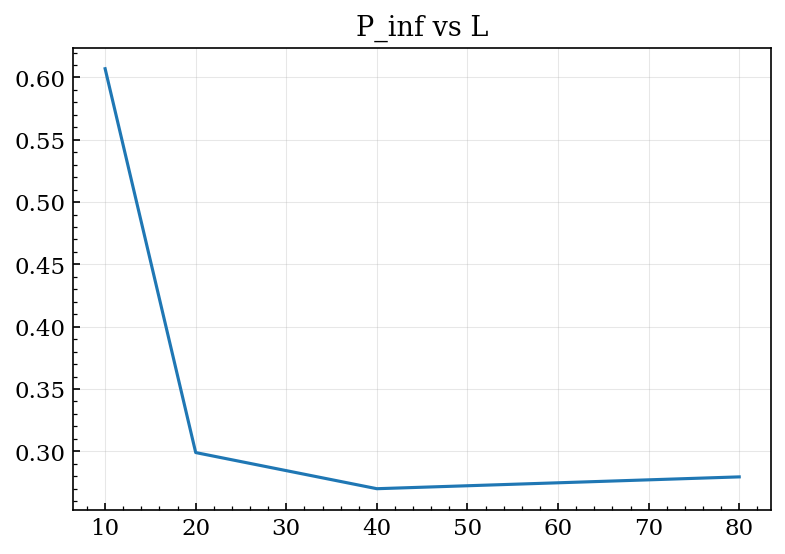
\includegraphics[width=0.5\linewidth]{PINFQ2.png}
\end{figure}
\begin{figure}[H]
    \centering
    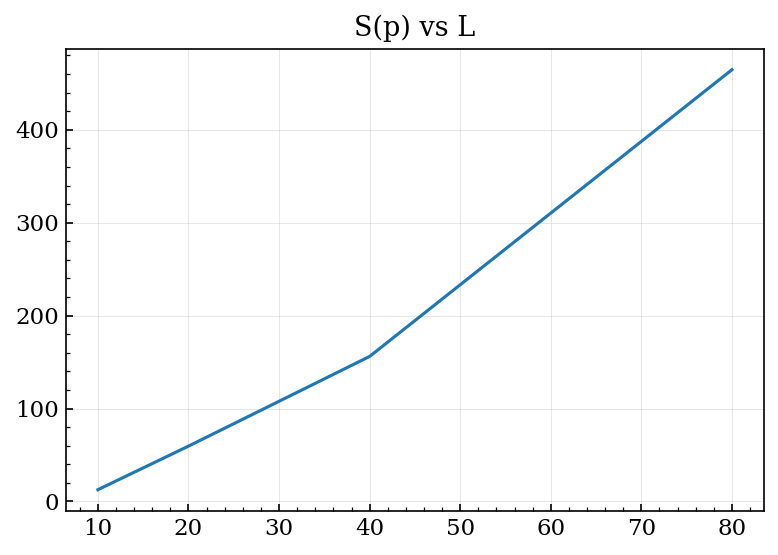
\includegraphics[width = 0.5\linewidth]{SPQ2.png}
\end{figure}
